\section{Anforderungen}

\subsection{Allgemeine Beschreibung}

\subsubsection{Produktperspektive}


\subsubsection{Produktfunktionen}


\subsubsection{Benutzer Charakteristik}


\subsubsection{Einschränkungen}



\subsection{Use Cases}

\subsubsection{Use Case Diagramm}
\begin{minipage}{\textwidth}

\begin{figure}[H]
	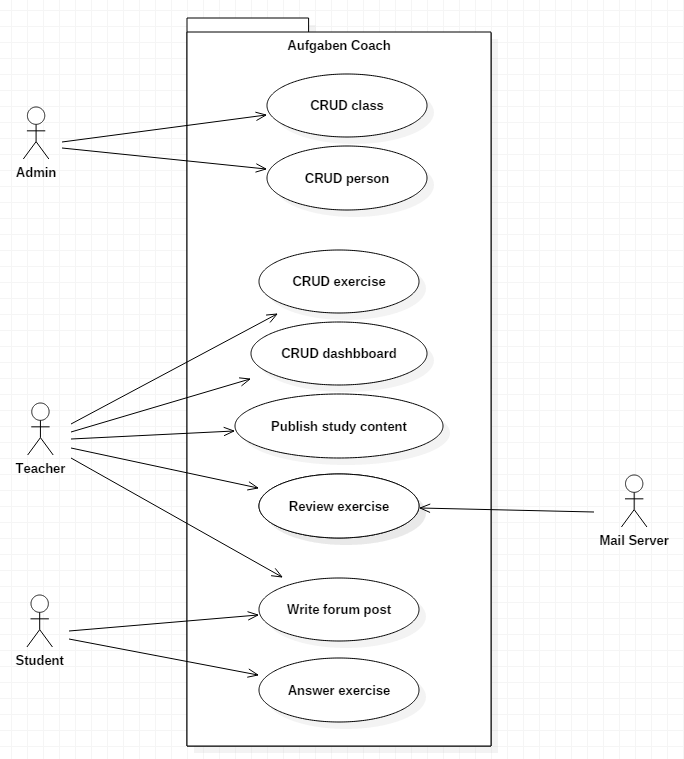
\includegraphics[width=\textwidth, height=\textheight, keepaspectratio]{images/UseCaseDiagramm.png}
	\caption{Use Case Diagramm}
\end{figure}

\end{minipage}


\begin{tabular}{| p{1cm} | p{1.3cm}|}
	\hline
	\textbf{Farbe} & \textbf{Priorität} \\
	\hline	
	grün & hoch \\
	\hline
	orange & tief \\
	\hline
\end{tabular}


\subsubsection{Aktoren}
Beschreibung der einzelnen Aktoren.
\newline
\begin{tabularx}{\textwidth}{| X | X |}
	\hline
		\textbf{Aktor} & \textbf{Beschreibung} \\
	\hline
		Administrator & Der Administrator ist für die Verwaltung der Klassen, Lehrer und Schüler zuständig. Er kann Klassen erstellen, Lehrpersonen und Schüler den Klassen zuweisen, etc. \\
	\hline
		Lehrer & Der Lehrer verwaltet die ihm zugewiesenen Klassen. Er kann Aufgaben erstellen und diese der Klasse zuweisen. Zusätzlich kann er Statistiken einsehen, die ihn über den aktuellen Wissensstand der Klasse informieren. \\
	\hline
		Schüler & Die Schüler haben Zugriff auf eine Wissensdatenbank und können Aufgaben und Quizzes, die ihnen zugewiesen wurden lösen. \\
	\hline
\end{tabularx}


\subsubsection{Beschreibung der Use Cases}
\textbf{UC01: CRUD person}

\noindent Hauptszenario: \\
Ein Administrator kann einen neuen Benutzer erstellen. Dabei kann er zwischen Lehrern und Schülern unterscheiden. Es müssen Angaben wie Vorname, Nachname, Benutzername, E-Mail Adresse und Passwort gemacht werden. Das System erstellt den gewünschten Benutzer, sodass dieser die Applikation ab sofort benutzen kann. \\

\noindent Alternatives Szenario: \\
Ein Administrator löscht eine nicht mehr berechtigte Person aus dem System. \\


\noindent \textbf{UC02: CRUD class}

\noindent Hauptszenario: \\
Ein Administrator erstellt eine neue Klasse. Dabei muss er den Namen der Klasse, wie auch das Eintrittsdatum angeben. Mit Hilfe des Eintrittsdatums kann im späteren Verlauf der Arbeit eine Statistik über mehrere ''Generationen'' von Klassen gemacht werden. \\

\noindent Alternatives Szenario: \\
Ein Administrator löscht eine nicht mehr benötigte Klasse aus dem System. \\


\noindent \textbf{UC03: assigne persons}

\noindent Hauptszenario: \\
Ein Administrator wählt eine bereits erstellte Klasse und weisst dieser eine unbestimmte Anzahl Lehrpersonen zu, sowie auch Schüler, welche noch keiner anderen Klasse zugewiesen wurden. \\

\noindent Alternatives Szenario: \\
Ein Administrator wählt eine bereits erstellte Klasse und entfernt Schüler und/oder Lehrer von dieser. \\


\noindent \textbf{UC04: CRUD exercise}

\noindent Hauptszenario: \\
Ein Lehrer definiert eine neue Aufgabe. Zur Aufgabe erstellt er mehrere Fragen. Zu jeder Frage kann er Hilfestellungen definieren, sowie angeben was die maximale Punktezahl ist. \\

\noindent Alternatives Szenario: \\
Ein Lehrer wählt eine erstellte Aufgabe aus und bearbeitet die Fragen dazu. Das heisst, es können weitere Fragen erstellt, bereits erstellte entfernt, oder aber auch neue Hilfestellungen hinzugefügt werden. \\


\noindent \textbf{UC05: CRUD weekly schedule}

\noindent Hauptszenario: \\
Ein Lehrer erstellt einen Wochenplan. Er erweitert Aufgaben und Quizzes mit einer Deadline und weisst diese einer seiner Klassen zu. \\

\noindent Alternatives Szenario: \\
Ein Lehrer bearbeitet einen bereits erstellten Wochenplan. Die Deadline einer Aufgabe wird um einen oder zwei Tage verschoben. \\


\noindent \textbf{UC06: CRUD quiz}

\noindent Hauptszenario: \\
Ein Lehrer definiert ein Quiz. Dazu erfasst er einige Fragen, die entsprechenden Antwortmöglichkeiten und die Lösungen. \\


\noindent \textbf{UC07: publish study content}

\noindent Hauptszenario: \\
Ein Lehrer schaltet ein neues Fach oder ein neues Thema für eine Klasse frei. \\

\noindent Alternatives Szenario: \\
Ein Lehrer entzieht einer Klasse das Recht ein Fach oder ein Thema zu sehen. \\


\noindent \textbf{UC08: view statistics}

\noindent Hauptszenario: \\
Ein Lehrer wählt eine Klasse und ein ihr zugewiesenes Fach aus. Das System berechnet anhand der von dieser Klasse gelösten Aufgaben eine Statistik und stellt diese dar. Wenn der Lehrer genauere Details sehen will, erstellt das System eine detailiertere Statistik. \\


\noindent \textbf{UC09: use forum}

\noindent Hauptszenario: \\
Ein Schüler sieht das aufgabenspezifische Forum. Findet er nicht die gewünschte Antwort, stellt er selber eine Frage. \\

\noindent Alternatives Szenario: \\
Ein Lehrer sieht, dass ein Schüler eine unbeantwortete Frage hat und beantwortet diese. \\


\noindent \textbf{UC10: send mail}

\noindent Hauptszenario: \\
Das System bemerkt, dass eine von einem Schüler gestellte Frage im Forum über längere Zeit nicht beantwortet wurde und informiert den Lehrer darüber per Mail. \\


\noindent \textbf{UC011: solve exercise}

\noindent Hauptszenario: \\
Ein Schüler löst eine Aufgabe. \\

\noindent Alternatives Szenario: \\
Ein Schüler überarbeitet eine bereits gelöste Aufgabe. \\


\noindent \textbf{UC012: solve quiz}

\noindent Hauptszenario: \\
Ein Schüler löst ein Quiz. \\

\noindent Alternatives Szenario: \\
Ein Schüler überarbeitet ein bereits gelöstes Quiz. \\


\subsection{Nicht Funktionale Anforderungen}
Im nachfolgenden Kapitel werden die nichtfunktionalen Anforderungen der Aufgaben-Coaching Applikation angesprochen.

\subsubsection{Qualität}
Um die Qualität des Codes möglichst hoch zu halten und sicherzustellen, dass alle Teammitglieder immer auf dem aktuellsten Stand sind, werden auf Git Pull-Requests verwendet. Dadurch kann sichergestellt werden, dass ein anderes Teammitglied den geschriebenen Code ebenfalls angesehen und durchdacht hat.

\subsubsection*{Maintainability}
Die Software könnte unter Umständen in einem Start-Up verwendet werden. Da in Zukunft noch beinahe beliebig viele neue Anforderungen hinzustossen können, soll die Applikation so gebaut werden, dass sie einfach modifiziert werden kann. 

\subsubsection*{Reliability}
Die Applikation soll robust und reibungslos laufen, auch wenn mehere Schüler zeitgleich mit der Plattform verbunden sind.

\subsubsection*{Scalability}
Das System soll problemlos von bis zu 300 Benutzern gleichzeitig verwendet werden können. 

\subsubsection*{Usability}
Bei der Applikation soll es sich um eine Mobile First Applikation handeln. Die Plattform soll sowohl auf Desktop PCs, Tablets und Smartphones bedienbar sein. Der Lehrer- und Administator-spezifische Teil der Applikation ist davon erstmals ausgenommen, da davon ausgegangen wird, dass diese beiden Aktoren hauptsächlich auf Desktop PCs arbeiten. 
Die Applikation soll ein intuitives User Interface besitzen, damit sich die Benutzer auf Anhieb zurechtfinden. 

\subsubsection*{Security}
Der Zugriff auf das System ist passwortgeschützt. Benutzer können sich nicht selbstständig registrieren. Nur Administratoren können neue Benutzer erfassen.
Jede Person sieht nur die Informationen, die für sie selbst von Bedeutung sind. Ein Schüler hat zum Beispiel keinen Zugriff auf die Statistiken anderer Schüler.


\newpage